% !TEX program = pdflatex
% Informe ejecutivo - Business Data Analytics Applied Lab #1
% Autor: Neyder Sebastian
% Compilar con: pdflatex Informe_Ejecutivo_Restaurante.tex
\documentclass[10pt,letterpaper]{article}

\usepackage[T1]{fontenc}
\usepackage[utf8]{inputenc}
\usepackage[spanish,es-nodecimaldot]{babel}
\usepackage{lmodern}
\usepackage[letterpaper,top=1.4cm,bottom=1.4cm,left=1.6cm,right=1.6cm]{geometry}
\usepackage{graphicx}
\usepackage{booktabs}
\usepackage{array}
\usepackage{xcolor}
\usepackage{tcolorbox}
\usepackage{enumitem}
\usepackage{titlesec}
\usepackage{caption}
\usepackage{multicol}
\usepackage{hyperref}
\usepackage{fancyhdr}
\usepackage{ragged2e}
\usepackage{siunitx}
\sisetup{output-decimal-marker={,},group-separator={.},group-minimum-digits=4}

\hypersetup{colorlinks=true,linkcolor=black,urlcolor=blue!60!black}

% ---------- Estilos ----------
\definecolor{brand}{HTML}{1F3A5F}
\definecolor{brandsoft}{HTML}{E8EEF6}
\definecolor{accent}{HTML}{59A14F}
\definecolor{warn}{HTML}{B26A00}

\titleformat{\section}
  {\color{brand}\bfseries\normalsize\uppercase}
  {}{0pt}{}[\vspace{-4pt}\color{brand}\hrule height 0.6pt\vspace{2pt}]
\titlespacing*{\section}{0pt}{4pt}{2pt}

\setlist[itemize]{leftmargin=1.1em,itemsep=0pt,topsep=1pt,parsep=0pt}
\setlength{\parindent}{0pt}
\setlength{\parskip}{2pt}
\captionsetup{font=small,labelfont={bf,color=brand},skip=2pt}
\renewcommand{\arraystretch}{1.05}

\pagestyle{fancy}
\fancyhf{}
\renewcommand{\headrulewidth}{0pt}
\fancyfoot[L]{\scriptsize\color{gray!70}Business Data Analytics -- Lab \#1 -- Semana 2}
\fancyfoot[R]{\scriptsize\color{gray!70}Datos: 500 registros, 2 semanas de operación}

\begin{document}

% ---------- Encabezado ----------
\begin{tcolorbox}[
    colback=brand,colframe=brand,arc=1pt,
    left=8pt,right=8pt,top=6pt,bottom=6pt,boxsep=0pt]
  \color{white}\bfseries\large
  DESEMPEÑO COMERCIAL Y ESTRATEGIA -- RESTAURANTE LA ANALÍTICA\\
  \color{white!85}\normalfont\small
  Informe Ejecutivo -- Semanas 1 y 2 \hfill Autor: Neyder Sebastián \hfill Data Analytics (43390860)
\end{tcolorbox}

\vspace{2pt}

% ---------- 1. Resumen Ejecutivo ----------
\section{1. Resumen Ejecutivo}

\begin{tcolorbox}[colback=brandsoft,colframe=brand!30,arc=1pt,
    left=6pt,right=6pt,top=4pt,bottom=4pt,boxsep=0pt]
\small
En dos semanas de operación se registraron \textbf{500 transacciones} por un total de
\textbf{\$3.886,56~USD}, con una variación de \textbf{-1,98\%} entre semanas
(\$1.962,68 $\rightarrow$ \$1.923,88). El hallazgo principal es una fuerte
\textbf{concentración de ingresos en un solo plato}: el \emph{Steak} explica $\sim$32\%
de los ingresos totales pese a ser apenas el 4.º producto por número de registros.
En paralelo, la \textbf{tasa de recurrencia} de clientes entre ambas semanas es de
\textbf{20,8\%} (46 de 221 clientes), lo que dimensiona una oportunidad clara de
fidelización.
\end{tcolorbox}

% ---------- 2. Desempeño del menú ----------
\section{2. Desempeño del Menú}

\begin{minipage}[t]{0.58\textwidth}
\vspace{0pt}
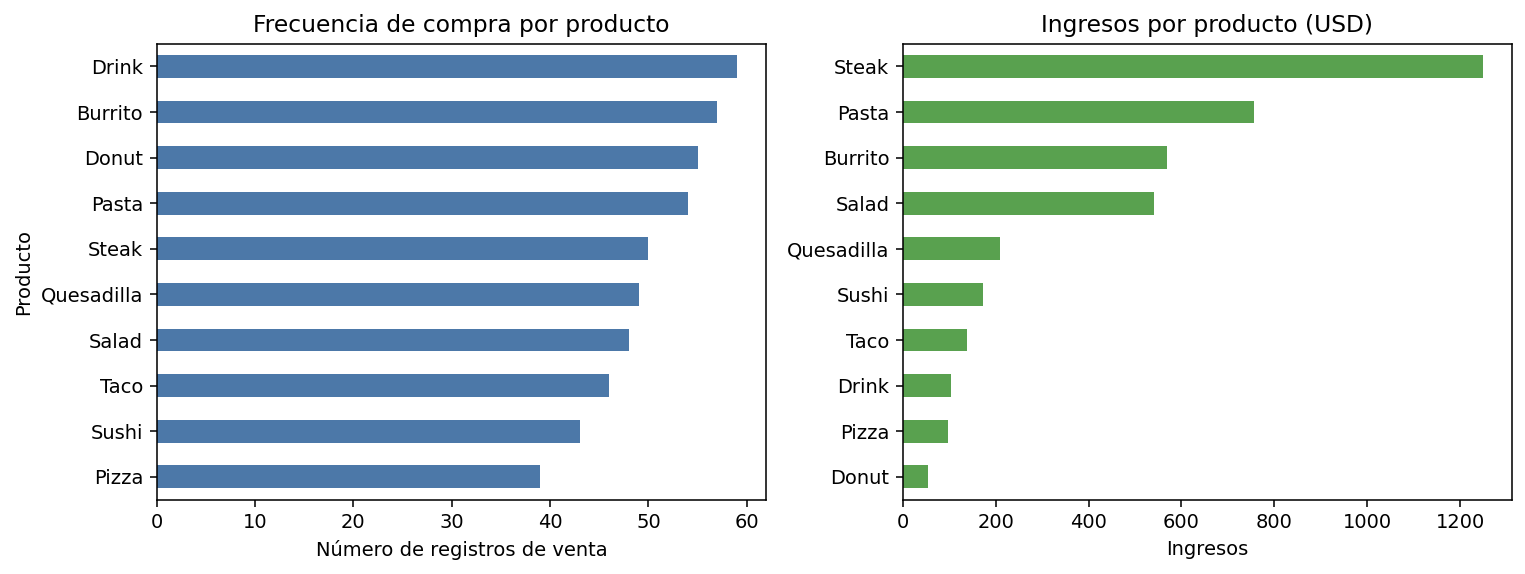
\includegraphics[width=\linewidth]{figuras/fig_menu.png}
\captionof{figure}{Frecuencia de compra frente a ingresos por producto. Los indicadores no son equivalentes.}
\end{minipage}\hfill
\begin{minipage}[t]{0.40\textwidth}
\vspace{0pt}
\footnotesize
\textbf{Producto de mayor ingreso:} \emph{Steak}, \$1.249,50 USD (50 registros).\\
\textbf{Producto más frecuente:} \emph{Drink}, 59 registros (\$103,25 USD).\\[2pt]
\textbf{Por qué no son equivalentes:} la frecuencia mide cuántas veces se pide un
plato; los ingresos combinan frecuencia con precio unitario. Un plato barato
puede liderar la frecuencia sin mover la caja, y un plato caro puede sostener
la caja con pocos pedidos. Leer los dos indicadores en paralelo evita
decisiones equivocadas: eliminar un plato por bajos ingresos podría reducir
el tráfico, y viceversa.\\[2pt]
\textbf{Segmentación operativa:} \emph{ancla de ingresos} = Steak, Pasta;
\emph{generadores de tráfico} = Drink, Donut, Pizza.
\end{minipage}

% ---------- 3. Comportamiento semanal ----------
\section{3. Comportamiento Semanal}

\begin{minipage}[t]{0.38\textwidth}
\vspace{0pt}
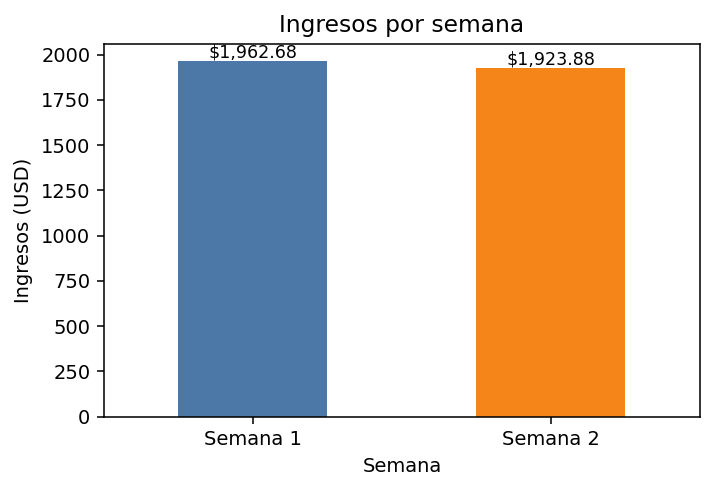
\includegraphics[width=\linewidth]{figuras/fig_semanal.png}
\captionof{figure}{Ingresos totales por semana.}
\end{minipage}\hfill
\begin{minipage}[t]{0.60\textwidth}
\vspace{0pt}
\footnotesize
\begin{center}
\begin{tabular}{lccc}
\toprule
\textbf{Semana} & \textbf{Registros} & \textbf{Ingresos (USD)} & \textbf{Prom. por registro} \\
\midrule
Semana 1 & 250 & \$1.962,68 & \$7,85 \\
Semana 2 & 250 & \$1.923,88 & \$7,70 \\
\midrule
\textbf{Variación} & \textbf{0} & \textbf{-\$38,80 (-1,98\%)} & \textbf{-\$0,16 (-2,0\%)} \\
\bottomrule
\end{tabular}
\end{center}
\vspace{2pt}
El volumen de operación fue idéntico (250 registros por semana). La caída de
ingresos ($-1,98\%$) proviene íntegramente de un ticket promedio ligeramente menor,
no de menor tráfico. \textbf{Con solo dos observaciones no puede afirmarse
tendencia ni atribuirse causa} (podría ser variabilidad natural, mezcla de
productos vendidos, o factores externos no medidos). Se requiere ampliar la
ventana para separar señal de ruido.
\end{minipage}

% ---------- 4 y 5 en dos columnas ----------
\section{4. Diagnóstico de Recurrencia \quad \& \quad 5. Perfil de Consumo y Recomendación Final}

\begin{minipage}[t]{0.55\textwidth}
\vspace{0pt}
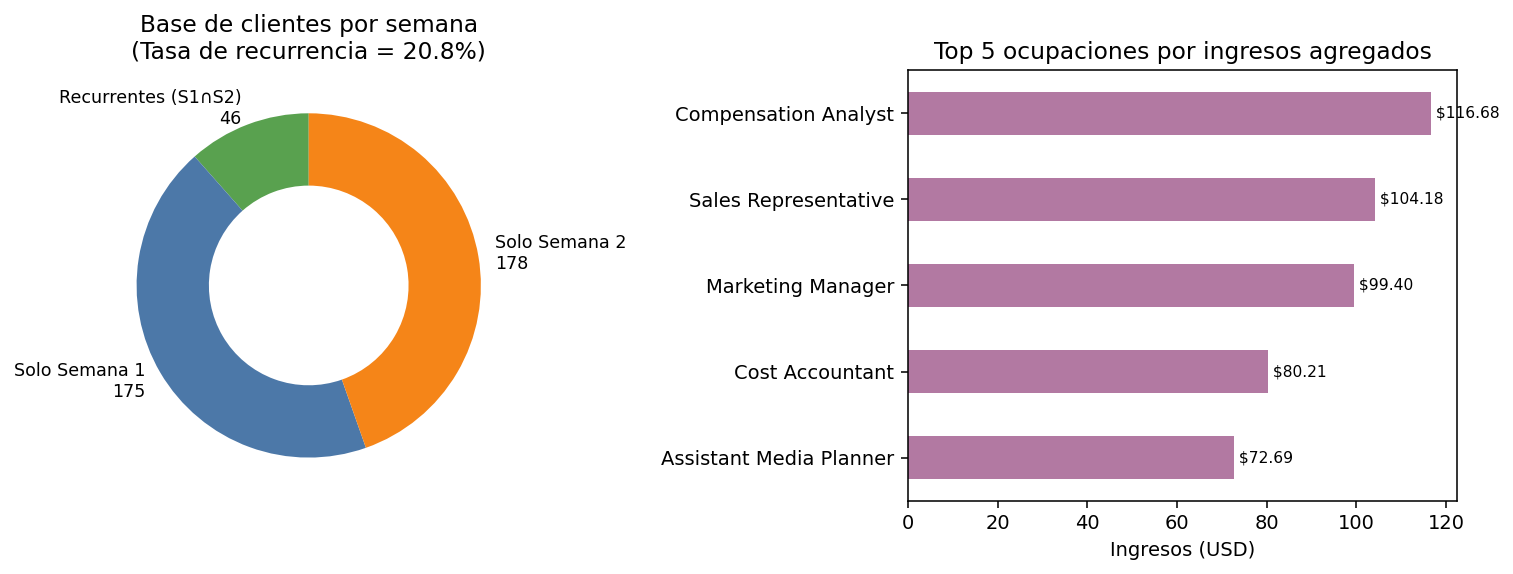
\includegraphics[width=\linewidth]{figuras/fig_recurrencia_ocupacion.png}
\captionof{figure}{Cohortes de clientes y ocupaciones con mayor gasto agregado.}
\end{minipage}\hfill
\begin{minipage}[t]{0.43\textwidth}
\vspace{0pt}
\footnotesize
\textbf{Recurrencia observada:} de \textbf{221} clientes únicos en la Semana 1,
\textbf{46 regresaron} en la Semana 2 $\rightarrow$ \textbf{tasa de recurrencia
20,8\%}. La Semana 2 sumó 178 clientes nuevos. La base es de alta rotación.\\[2pt]
\textbf{Acción de fidelización propuesta:} programa de \emph{segunda visita}
(cupón nominal de descuento o bebida cortesía) activado automáticamente tras
la primera compra, con vigencia de 7 días. Meta operativa: elevar la
recurrencia de \textbf{20,8\%} hacia \textbf{25--30\%} en la siguiente ventana.\\[2pt]
\textbf{Perfil agregado por ocupación (Top 5):}
Compensation Analyst (\$116,68), Sales Representative (\$104,18),
Marketing Manager (\$99,40), Cost Accountant (\$80,21),
Assistant Media Planner (\$72,69). \emph{Ninguna categoría concentra una
cuota dominante} y las muestras por ocupación son pequeñas: los patrones son
descriptivos y no soportan afirmaciones sobre clientes individuales.\\[2pt]
\textbf{Recomendación prioritaria:} activar el programa de segunda visita,
proteger disponibilidad y visibilidad del \emph{Steak} (ancla de ingresos) y
mantener el precio de los generadores de tráfico como palanca de recurrencia.
Todo se optimiza \textbf{por ingresos y reincidencia}, no por margen, porque
los datos no contienen costos.
\end{minipage}

% ---------- Franja de limitaciones ----------
\vspace{2pt}
\begin{tcolorbox}[colback=warn!8,colframe=warn!40,arc=1pt,
    left=6pt,right=6pt,top=3pt,bottom=3pt,boxsep=0pt]
\scriptsize
\textbf{Alcance y limitaciones.} Los datos disponibles son precios de venta unitarios,
sin costos, cantidades, descuentos, marca temporal (día/hora), canal ni ticket agrupado
por visita. En consecuencia, este informe analiza \textbf{ingresos, frecuencia y
recurrencia}, y no habla de \textbf{rentabilidad, utilidad ni margen}. Dos semanas de
observación no permiten afirmar tendencia ni causalidad. Cifras validadas con
\texttt{assert} sobre unicidad y referencias, y con contraste \texttt{Pandas vs SQL}.
Se omiten nombres de clientes por privacidad.
\end{tcolorbox}

\end{document}
